\chapter{Iteracion 7: Caso de prueba con un sensor de campo electrostatico} % (fold)
\label{cha:iteracion_7}

\section{Introduccion} % (fold)
\label{sec:introduccion}

Parte de este proyecto fue poner a prueba nuestro sistema utilizando un sensor detector de campo electrostatico. Ademas de obtener las mediciones, fue necesario realizar un sistema de control para el motor del sensor. En esta iteracion realizamos la adaptacion necesaria de los requisitos de funcionamiento del sensor a nuestro sistema de instrumentacion, probando asi el funcionamiento del mismo, asi como tambien el funcionamiento del sistema gestionador desarrollado en la iteracion \ref{cha:iteracion_6} 

\subsection{Marco teorico} % (fold)
\label{sub:marco_teorico}

La intensidad de un campo electrico se puede medir, en principio, colcando un medidor de voltaje entre dos placas metalicas paralelas separadas por una distancia. El problema de esto es que, como el medidor de voltaje suele tener una impedancia alta en la entrada, cualquier voltaje inducido en las placas se pierde rapidamente, y no podria usarse para medir el capo electrico. Para arreglar esto, se utiliza la tecnica de las aspas. Se coloca una placa conductora, y sobre la misma se posiciona un sistema con aspas de forma que cuando estas roten, se cubra y se exponga periodicamente la placa conductora al campo electrico ambiental. Para lograr esto apropiadamente, el rotor que hace girar las aspas debe estar conectado a tierra. La placa conductora esta conectada a tierra a traves de un amplificador de transconductancia, que convierte la corriente que va desde la placa a tierra en una tension.
A medida que la placa conductora este expuesta al campo electrico, el campo induce una corriente a tierra mientras que atrae o repele la carga de la placa conductora. A medida que la placa esta cubierta del campo electrico, la carga inducida se drena. Entonces las placas inducen una corriente alterna a masa que es proporcional a la intensidad del campo electrico estatico. Esta corriente alterna luego puede ser rectificada para utilizarla como entrada a un conversor analogico digital y obtener asi la intensidad del campo electrico medido. \\

Una vez obtenida la intensidad, es necesario saber el signo del campo electrico medido. Para obtenerlo, un metodo es que en el mismo conversor analogico digital se obtenga la medicion de manera diferencial. Un conversor analogico digital diferencial toma la diferencia entre dos canales para obtener un dato en lugar de tomar el valor de un canal y compararlo con tierra. De forma que es posible determinar cual es el canal con mayor tension. Con esto, se pueden conectar los canales de las señales de tierra y la de la placa conductora, y se miden de manera diferencial para obtener tento la intensidad como el signo del campo electrico estatico.
\cite{sensorcampo}

% subsection marco_teorico (end)
\subsection{El sensor} % (fold)
\label{sub:el_sensor}

El sensor utilizado es un dispositivo que mide la intensidad del campo electrico en el ambiente debido al campo electrostatico generado por la carga electrica de las nubes en el momento. Se puede utilizar para detectar la posibilidad de que caiga un rayo en una zona cercana al sensor, y tambien para investigar los efectos de la electricidad estatica. Para funcionar, el sensor necesita de un motor que gire a velocidad constante. Este motor funciona en base a un driver que tiene como entrada una señal modulada por ancho de pulso.
Mientras el motor gire a velocidad constante, es posible obtener datos validos del sensor. La idea es hacer que el funcionamiento del sensor como la adquisicion de las mediciones sea logrado con funcionalidades de la placa de instrumentacion, mas otras caracteristicas que ofrece el microcontrolador C8051F352, como ser el modulo de PWM para generar la señal modulada por ancho de pulso, y el uso de los timers para establecer las bases de tiempo que utilizamos para hacer un control de estabilidad en la velocidad del motor. \\

Fisicamente, es una estructura metalica compuesta por un motor que hace girar unas aspas que se se encargan de blindar y desblindar una placa que a su vez se carga y descarga con la electricidad estatica del ambiente. esta carga y descarga continua es lo que justamente se termina transformando en el nivel de voltaje que nos indica el nivel de electricidad estatica del ambiente, que es lo que queremos saber.
La placa y las aspas funcionan como un capacitor que se blinda y se des\-blinda a medida que el motor gira. En el momento que las aspas estan descuburiendo la placa, el capacitor se carga, y en el momento que se cubre la placa, el capacitor se descarga. La descarga se hace sobre un amplificador que luego va a un conversor analogico digital, que termina en la lectura de un valor que nos dice el nivel del campo electrostatico ambiental. En el caso particular de este sensor, el motor que hace girar las aspas es un motor brushless manejado por un driver PWM.

\begin{figure}[h]
  \centering
  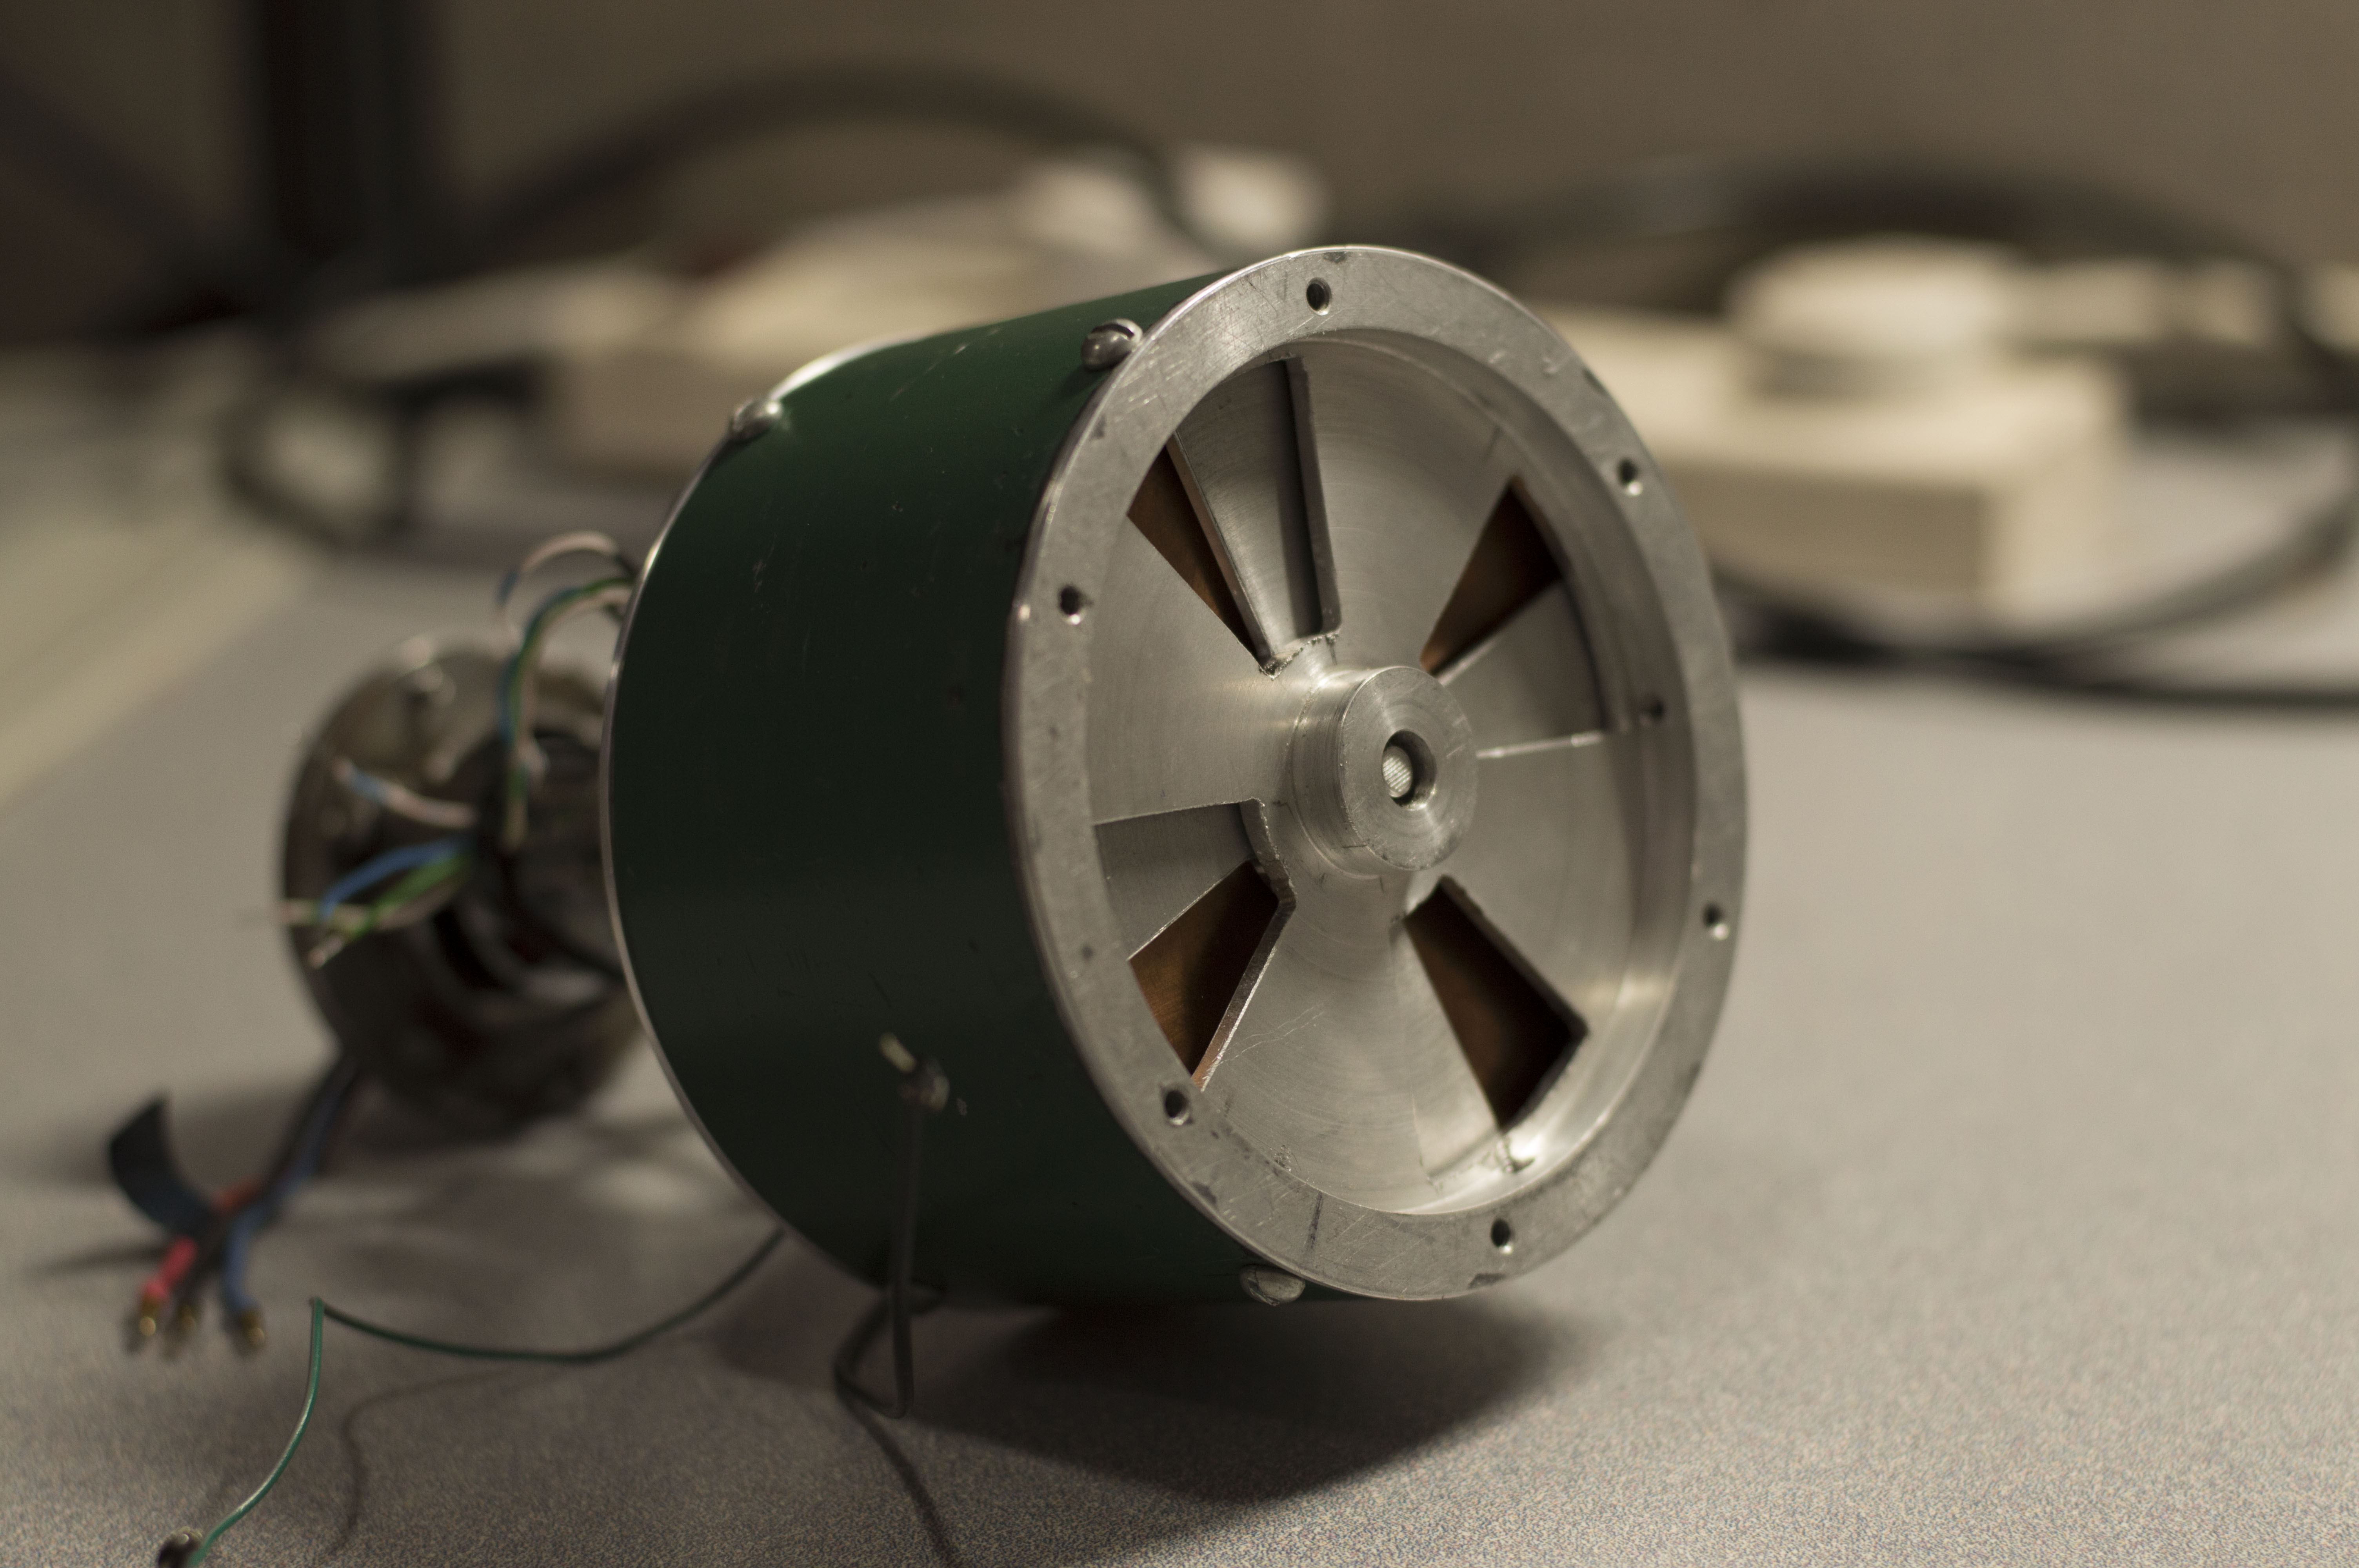
\includegraphics[width=0.80\textwidth, height = 7cm]{sensorhorizontal}
  \caption[Imagen del sensor de campo electrostatico utilizado (horizontal)]{Foto del sensor en horizontal. Las aspas que pueden verse son las responsables de cubrir y descubrir la placa cargada (color cobre), que es la que se carga con la electricidad estatica del ambiente.}\label{fig:sensorhorizontal}
\end{figure}

\begin{figure}[h]
  \centering
  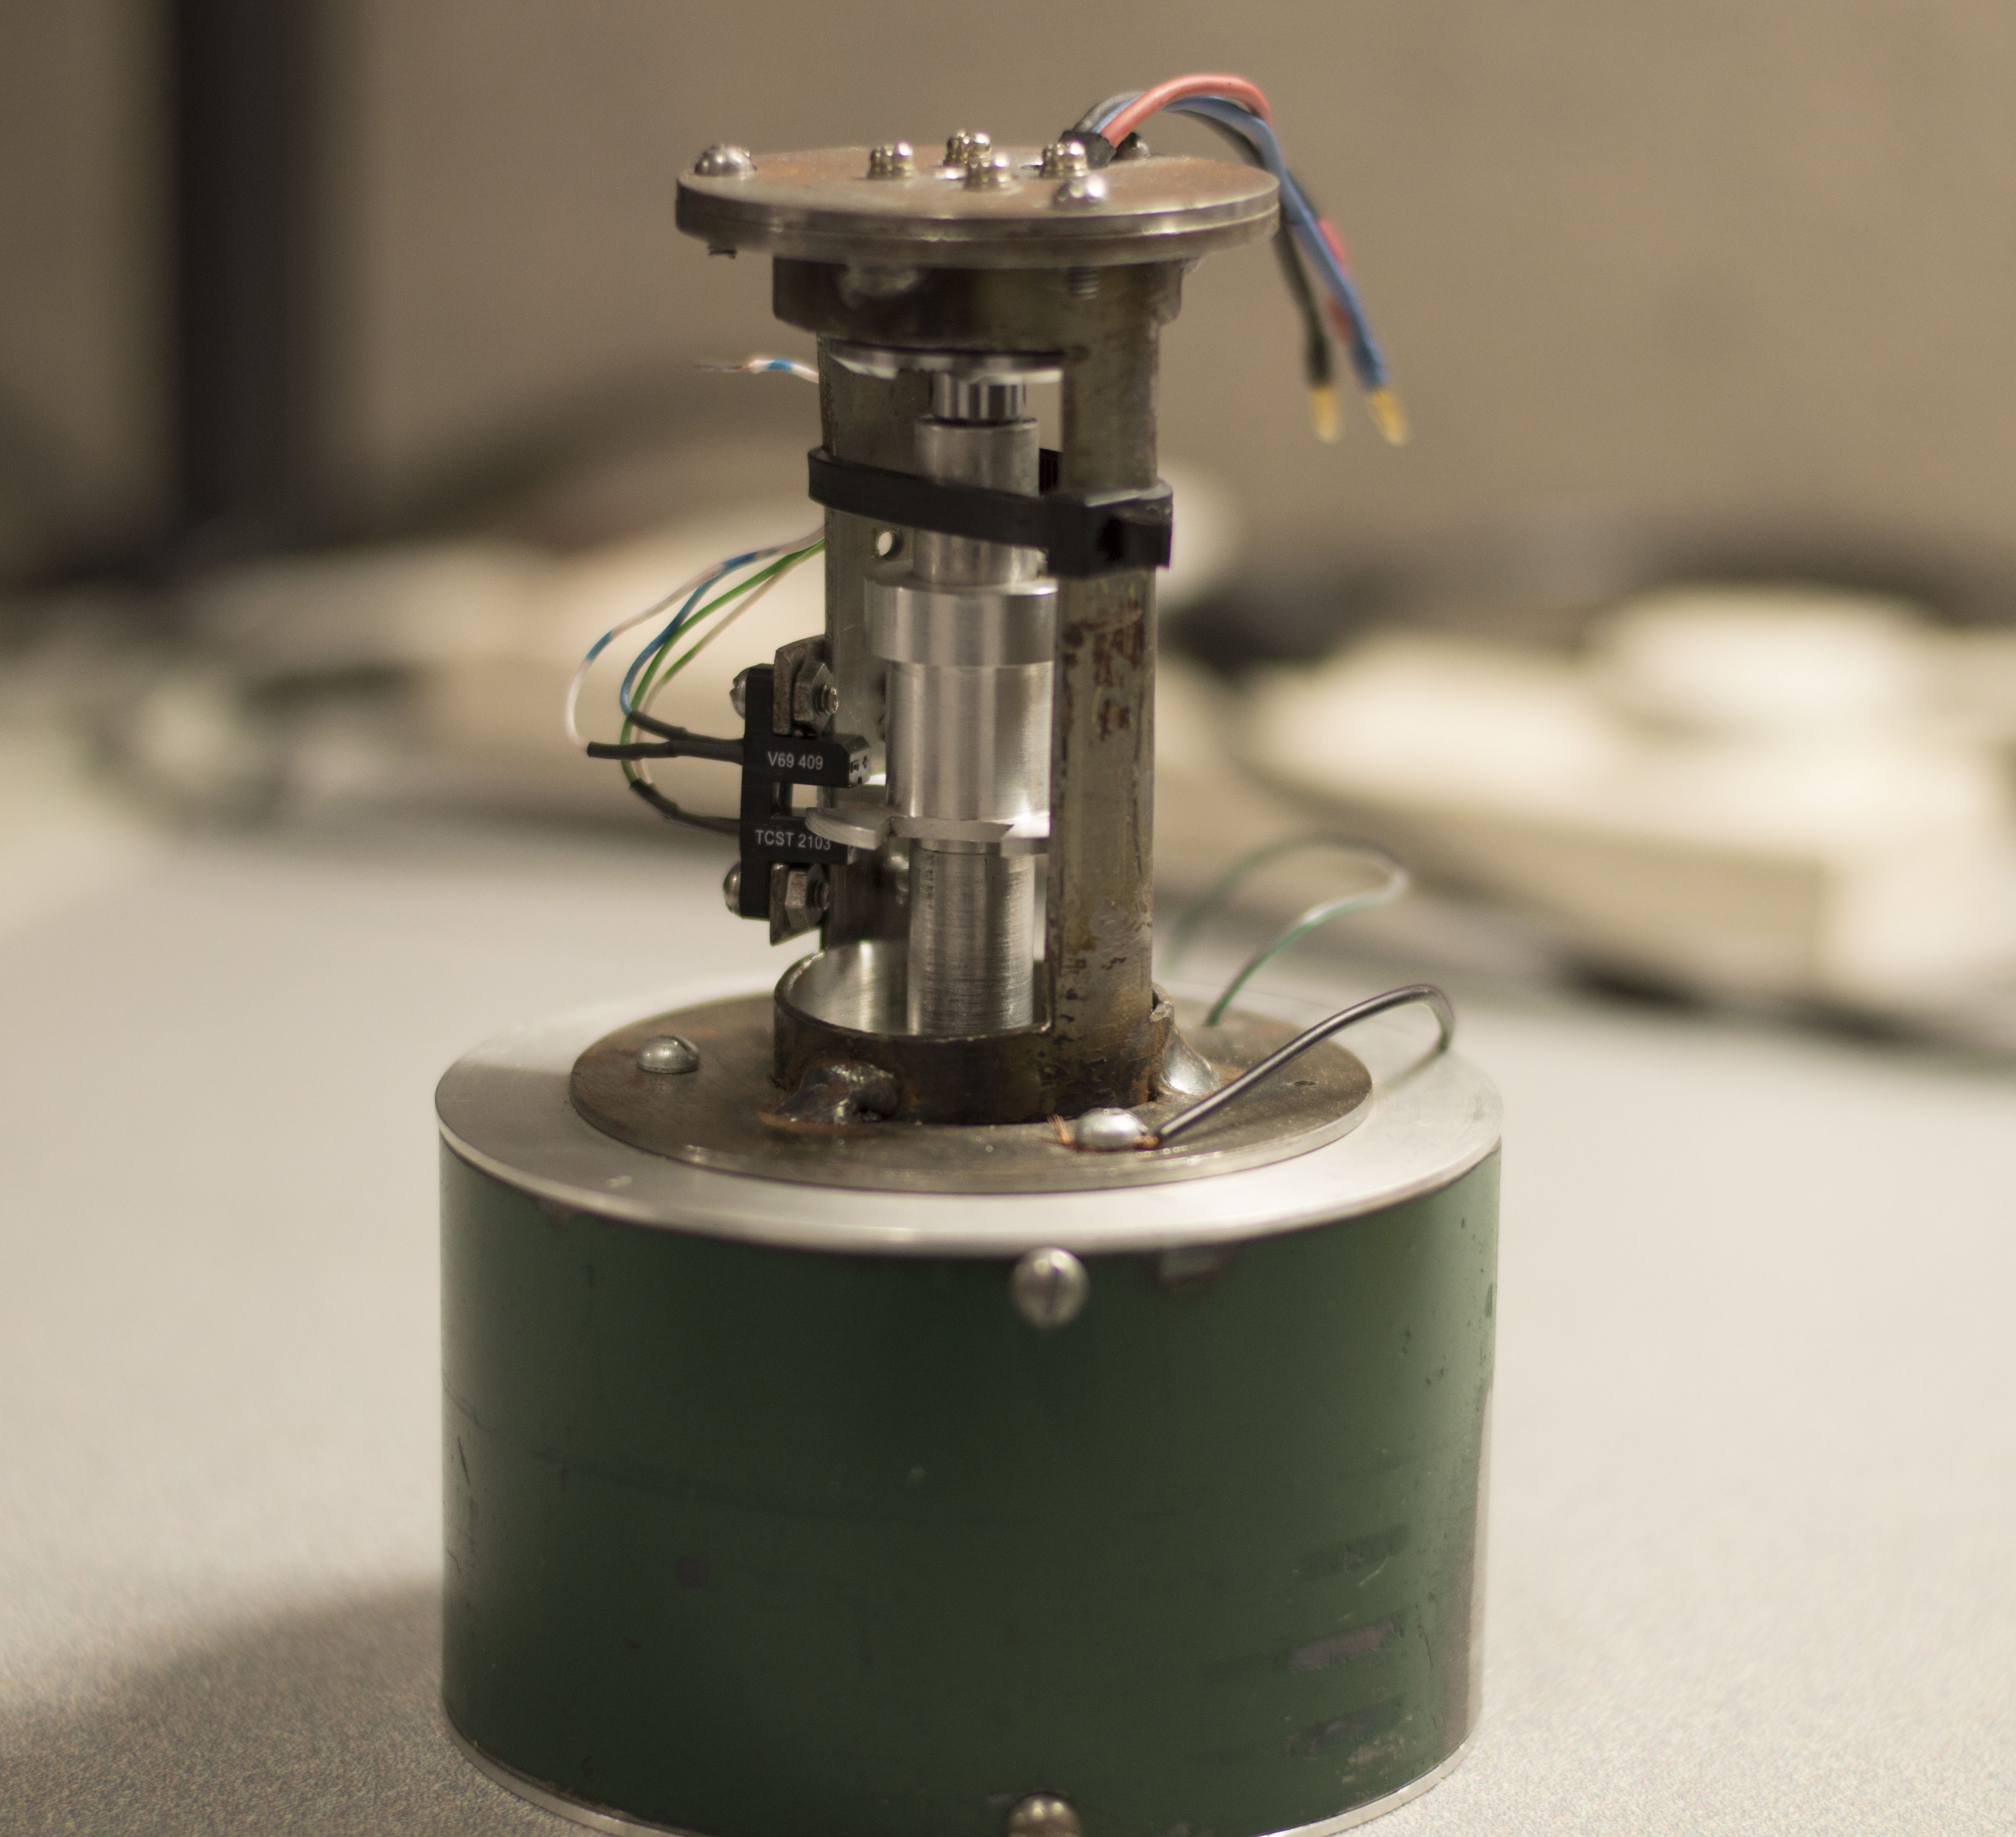
\includegraphics[width=0.80\textwidth, height = 7cm]{sensorvertical}
  \caption[Imagen del sensor de campo electrostatico utilizado (vertical)]{Foto del sensor en vertical. Puede verse en el eje, el sistema de aspas y fotointerruptor utilizado para medir las RPM.}\label{fig:sensorvertical}
\end{figure}

Ademas de las aspas que miden el campo electrico, en el eje del motor se encuentra un segundo grupo de aspas, pero mas pequeño; junto a estas aspas se encuentra acoplado un fotointerruptor, de manera que el paso de cada aspa interrumpe el paso de luz de un extremo a otro. Si se construye el circuito requerido para el fotointerruptor, ocurrira que cuando el motor este girando, se generen pulsos cuadrados a la salida del fotointerruptor, permitiendo obtener cuentas que ayudaran a la hora de controlar la velocidad del motor. Las aspas secundarias y el fotointerruptor pueden verse en la figura \ref{fig:sensorvertical}

% subsection el_sensor (end)

% section introduccion (end)

\section{Requerimientos de la iteracion} % (fold)
\label{sec:requerimientos_de_la_iteracion}

\begin{itemize}
\item Se deberian utilizar las funcionalidades de los sistemas desarrollados en el transcurso del proyecto para obtener mediciones del sensor
\item Se deberia controlar la velocidad del motor utilizando el fotointerruptor
\item Se deberia diseñar y construir una placa con un circuito de adaptacion para el funcionamiento y la operacion del sensor
\item La placa de adaptacion deberia poder ser acoplable a la placa de instrumentacion (como shield)
\item Se deberia construir un recipiente donde pueda entrar el sensor junto con el sistema de instrumentacion y el sistema gestionador, para poder colocarlo en el aire libre con el objetivo de realizar una prueba de campo
\end{itemize}


% section requerimientos_de_la_iteracion (end)

\section{Experimentacion} % (fold)
\label{sec:experimentacion}

El motor dentro de este sensor incluia un driver PWM. Para arrancar y dar velocidad a este motor, se utilizo, como primera instancia, una placa de desarrollo Arduino con un software hecho por Emiliano Pellicioni y Diego Gutierrez. Con el driver conectado a la placa y el programa funcionando, era posible arrancar el motor y darle una velocidad (aunque no muy constante).

Teniendo el motor funcionando, la teoria indica que el sensor esta midiendo campo. Para probar esto, se utilizo una regla de plastico cargada con electricidad estatica y un osciloscopio conectado a la salida del sensor. Al acercar y alejar la regla de las aspas, se podia ver en la salida del osciloscopio como la onda resultante a la salida del sensor aumentaba y disminuia en amplitud. Lo que estabamos viendo, en ese momento, era una salida ``en crudo'' del sensor. Para poder convertir la señal y obtener datos coherentes, era necesario rectificar la señal. \\

El fotointerruptor acoplado al eje del motor da la posibilidad de realizar un conteo de señales cuadradas que nos proporcione los datos suficientes como para realizar una medicion de las vueltas por minuto del motor. Necesita de un circuito basico para funcionar. Lo construimos en una protoboard junto con todo lo necesario para hacer funcionar el motor. Con ayuda de un osciloscopio, fue posible ver los pulsos cudadrados de 5 Volts generados por el fotointerruptor. Estos pulsos son los que luego servirian de entrada a un contador de eventos de la placa de instrumentacion, con el objetivo de controlar la velocidad del motor. \\

ACA FALTARIA INCLUIR IMAGENES DE:

-EL OSCILOSCOPIO CON LA SALIDA DEL SENSOR MIDIENDO
-EL OSCILOSCOPIO CON LA SALIDA DEL FOTO INTERRUPTOR

% section experimentacion (end)

\section{Implementacion de una placa de adaptacion para el sensor de campo} % (fold)
\label{sec:implementacion_de_una_placa_de_adaptacion_para_el_sensor_de_campo}

Para el debido funcionamiento y control del sensor, se planteo en los requerimientos el desarrollo de una placa con que contenga los circuitos necesarios para alimentar el motor, tratar la señal de medicion de campo, y tratar los pulsos cuadrados del fotointerruptor, de forma que la placa de instrumentacion pueda leer ya procesados los datos necesarios para medir el campo y controlar la velocidad del motor.


\subsection{Requerimientos} % (fold)
\label{sub:requerimientos}

A partir de estas pruebas sacamos las siguientes conclusiones para el circuito de adaptacion del sensor:

\begin{itemize}
	\item Debe poder conectarse la alimentacion y las entradas PWM del driver del motor
	\item Debe incluir un circuito de adaptacion (rectificacion y amplificacion) de la señal del sensor
	\item Debe incluir el circuito necesario para el funcionamiento del fotosensor.
	\item El diseño de la placa deberia ser tal que sea acoplable y desacoplable a la placa de instrumentacion.
\end{itemize}

Mediante investigacion y prueba y error, se desarrollaron los circuitos necesarios para cumplir con estos requerimientos y se fusionaron en un unico circuito que luego iria impreso en una placa. Para mejorar la practicidad, la placa deberia poder ser acoplable y desacoplable a la placa de instrumentacion. Esto ultimo se tuvo en cuenta a la hora de diseñar el despliegue de componentes y las dimensiones de la placa.

% subsection requerimientos (end)
\subsection{Circuito de adaptacion para la señal de nivel de campo} % (fold)
\label{sub:circuito_de_adaptacion_para_la_señal_de_nivel_de_campo}

aca va el operacional con el amplificador y rectificador que se pone para que vaya antes del conversor.. con imagen

% subsection circuito_de_adaptacion_para_la_señal_de_nivel_de_campo (end)

\subsection{Circuito de adaptacion para la señal de pulsos del fotointerruptor} % (fold)
\label{sub:circuito_de_adaptacion_para_la_señal_de_pulsos_del_fotointerruptor}

La figura \ref{fig:fotointerruptorcircuitotipico} muestra el circuito que implementamos para el fotointerruptor. Es un diseño tipico utilizado en la mayoria de los casos en los que se utiliza este tipo de sensor. 

\begin{figure}[h]
  \centering
  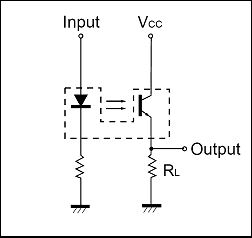
\includegraphics[width=0.80\textwidth, height = 7cm]{fotointerruptorcircuitotipico}
  \caption{Circuito utilizado para el fotointerruptor}\label{fig:fotointerruptorcircuitotipico}
\end{figure}

En esta disposicion, cuando el fotosensor esta iluminado, hay 5 Volts en la salida; de lo contrario 0 Volts. Esto hace que cuando el motor gira, las aspas van a tapar y destapar la entrada de luz al fotosensor generando una onda cuadrada a la salida del circuito, cuya frecuencia depende de la velocidad del motor.
Esta señal se utiliza como entrada para el contador de eventos, luego en el programa se calcula la velocidad del motor utilizando las cuentas obtenidas sobre una base de tiempo. 

% subsection circuito_de_adaptacion_para_la_señal_de_pulsos_del_fotointerruptor (end)

\subsection{Circuito de alimentacion} % (fold)
\label{sub:circuito_de_alimentacion}

La placa de instrumentacion esta diseñada para estar siempre encendida. Al no consumir mucho, no trae problemas de consumo o temperatura. Pero habiendo hecho esta adaptacion, era necesario tener en cuenta el consumo del motor mientras esta encendido pero sin girar. Para ahorrar consumo, propusimos agregar un control de encendido y apagado del sensor, utilizando uno de los pines GPIO del microcontrolador. \\

La figura PONER FIGURA DEL CIRCUITO muestra el circuito que prepara la señal del microcontrolador que controla el encendido y apagado del motor. Utilizamos un relé, un optoacoplador, un transistor, un diodo y resistencias. El optoacoplador sirve para aislar opticamente el circuito logico del motor con el circuito de 12 V. El rele electromecanico conmuta la conductividad entre el motor y masa, de manera que en un estado del rele el motor esta prendido, y en el otro esta apagado. Utilizamos un transistor porque los 5V a la salida del optoacoplador no eran suficientes para la tension de switching del relé.

% subsection circuito_de_alimentacion (end)

\subsection{Señal modulada en ancho de pulso para el driver del motor} % (fold)
\label{sub:señal_modulada_en_ancho_de_pulso_para_el_driver_del_motor}

% aca en realidad no hicimos nada porque lo unico que hay es el cable de salida del pwm que viene de la placa y se conecta de pecho al driver.. pero bueno explicar eso.. y explicar tambnein que pasamos desde el arduino que hacia todo por interrupciones al pwm de la placa que lo hace todo por HW y funciona mucho mejor. aunque no explicar como funciona el programa porque eso va despues

El driver del motor funciona a base de señales moduladas en pulso. Los anchos de pulso funcionan como codigos que representan distintos modos para el driver. El manual del driver especifica los distintos anchos de pulso que lo configuran de distintas maneras. Para guiarse en el proceso de configuracion, el driver suena con distintos ``beeps'' de distintos tonos que indican distintas cosas.

En nuestro caso, necesitabamos arrancar el motor y hacerlo a andar a una unica velocidad. Lo cual es uno de los modos mas simples. De igual manera, era necesario una serie de señales sucesivas con distintos anchos de pulso para arrancar el motor. Estas señales las hicimos utilizando un modulo del microcontrolador denominado PCA.





% subsection circuito_de_adaptacion_para_la_señal_modulada_en_ancho_de_pulso_para_el_driver_del_motor (end)

\subsection{Circuito final} % (fold)
\label{sub:circuito_final}


% subsection circuito_final (end)

% section implementacion_de_una_placa_de_adaptacion_para_el_sensor_de_campo (end)


\section{Funcionalidades desarrolladas dentro del software de la placa de instrumentacion para trabajar junto con el sensor} % (fold)
\label{sec:funcionalidades_desarrolladas_dentro_del_software_de_la_placa_de_instrumentacion_para_trabajar_junto_con_el_sensor}

Al programa embebido en el microcontrolador, le agregamos funcionalidades especificas para trabajar con este sensor. Realizamos un modulo aparte llamado sensor, cuyas funciones estan desarrolladas especificamente para este sensor y no otro. Estas funciones incluyen:

\begin{itemize}
	\item Dar arranque y parada al motor
	\item Establecer una velocidad al motor
	\item Controlar la velocidad del motor.
\end{itemize}

La medicion en si de los datos del sensor no esta como funcion especifica del mismo porque ya se cubre con las funciones ya hechas en el modulo del conversor.

\begin{figure}[h]
  \centering
  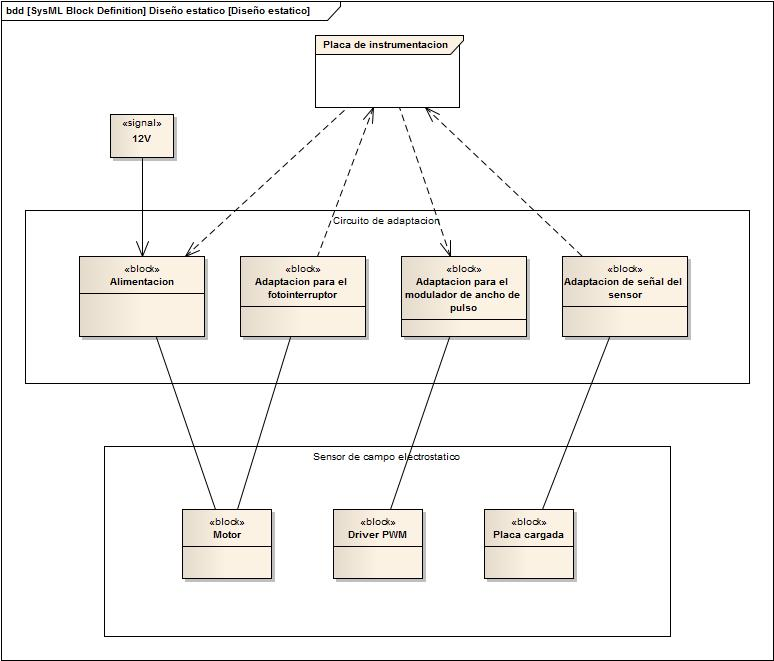
\includegraphics[width=0.80\textwidth, height = 7cm]{diagramabloquessensor}
  \caption{Diagrama de bloques fisicos del sistema de adaptacion del sensor}\label{fig:diagramabloquessensor}
\end{figure}

Y DE ACTIVIDAD PARA BER LA SUCESION DE COSAS QUE OCURREN CUANDO SE:
-PRENDE EL MOTOR
-SE CONTROLA VELOCIDAD

MAS QUE NADA.. ES LO MAS IMPORTANTE.

% section funcionalidades_desarrolladas_dentro_del_software_de_la_placa_de_instrumentacion_para_trabajar_junto_con_el_sensor (end)

\section{Pruebas} % (fold)
\label{sec:pruebas}

% section pruebas (end)

\section{Resultados} % (fold)
\label{sec:resultados}

% section resultados (end)

% chapter iteracion_7 (end)